\documentclass[english]{article}
\usepackage[T1]{fontenc}
\usepackage[latin9]{inputenc}
\usepackage{varwidth}
\usepackage{tikz}
\usetikzlibrary{shapes.geometric, arrows}

%define styles
\tikzstyle{body} = [rectangle, rounded corners, minimum width=3cm, minimum height=1cm,text centered, draw=black!50, fill=blue!10]

\tikzstyle{head} = [rectangle, minimum width=3cm, minimum height=1cm, text centered, draw=black!50, fill=yellow!25]

\tikzstyle{arrow} = [thick,->,>=stealth]
\tikzstyle{arrowr} = [thick,<-,>=stealth]



\begin{document}

\pagenumbering{gobble}

%\section{A machine-learning project flow chart}

\begin{figure}[!h]
\centering
\caption{A visual guide to illustrate steps involved in a machine-learning project.}
\vspace{5mm}
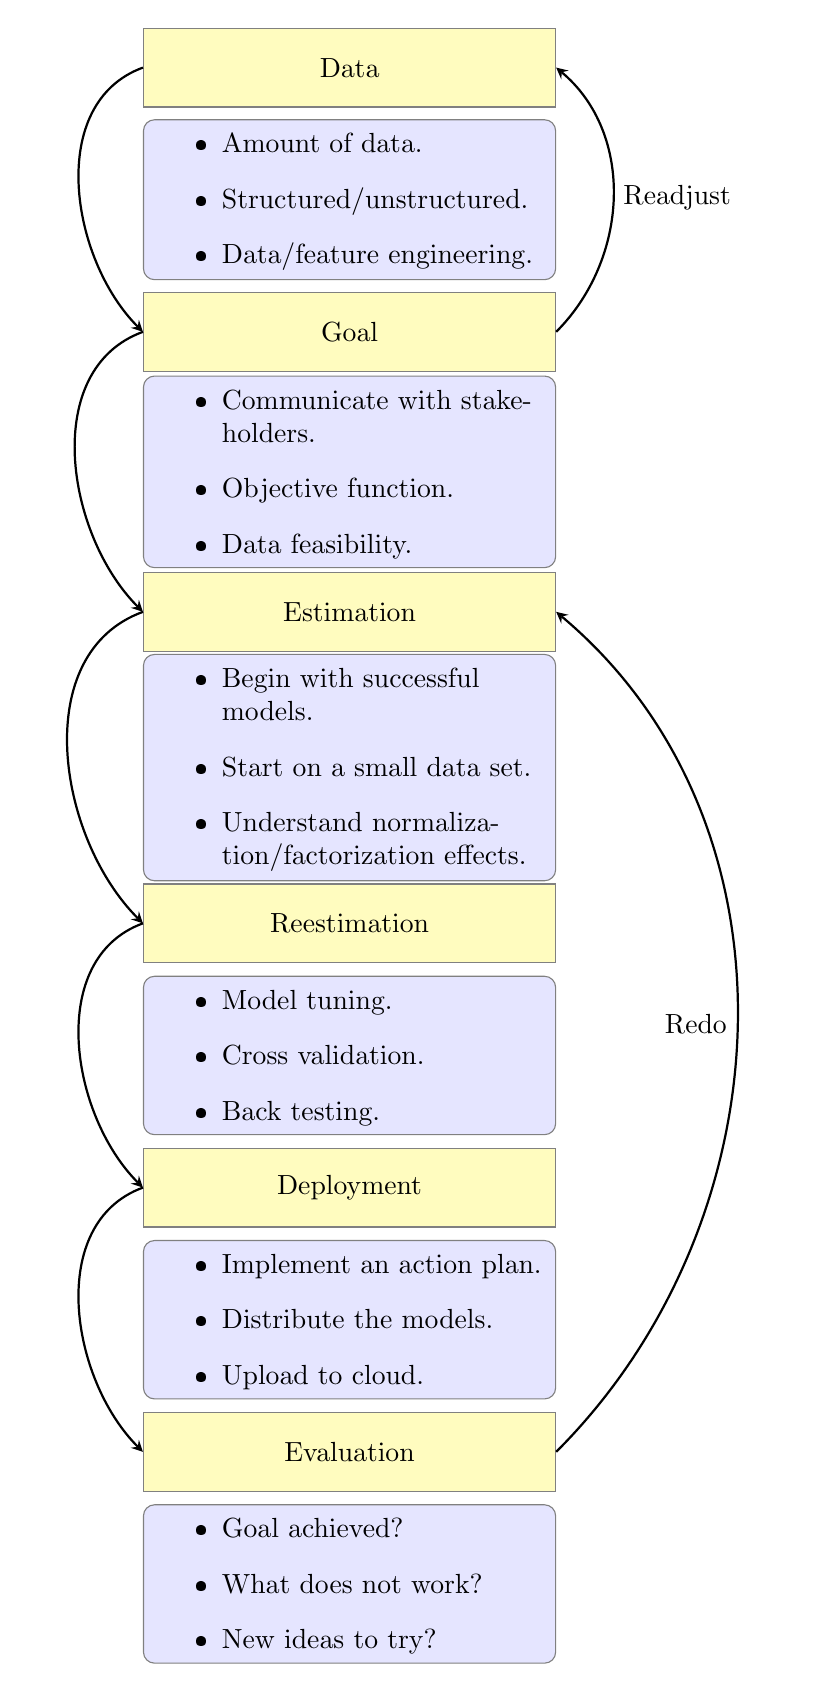
\begin{tikzpicture}[node distance=.7in]

%Data
\node (data_head) [text width=5cm, head] {Data};

\node (data_body) [text width=5cm, body, below of=data_head, yshift=.1cm] {
\vspace{-4mm}
\begin{itemize}
\item Amount of data.
\item Structured/unstructured.
\item Data/feature engineering.

\end{itemize}};

%Goal
\node (goal_head) [text width=5cm, head, below of=data_body, yshift=.1cm] {Goal};
\node (goal_body) [text width=5cm, body, below of=goal_head] {
\vspace{-4mm}
\begin{itemize}
\item Communicate with stakeholders.
\item Objective function.
\item Data feasibility.
\end{itemize}};

%Estimation
\node (estimation_head) [text width=5cm, head, below of=goal_body] {Estimation};
\node (estimation_body) [text width=5cm, body, below of=estimation_head, yshift=-.2cm] {
\vspace{-4mm}
\begin{itemize}
\item Begin with successful models.
\item Start on a small data set.
\item Understand normalization/factorization effects.
\end{itemize}};

%Reestimation
\node (reestimation_head) [text width=5cm, head, below of=estimation_body, yshift=-.2cm] {Reestimation};
\node (reestimation_body) [text width=5cm, body, below of=reestimation_head, yshift=.1cm] {
\vspace{-4mm}
\begin{itemize}
\item Model tuning.
\item Cross validation.
\item Back testing.
\end{itemize}};

%Deployment
\node (deployment_head) [text width=5cm, head, below of=reestimation_body, yshift=.1cm] {Deployment};
\node (deployment_body) [text width=5cm, body, below of=deployment_head, yshift=.1cm] {
\vspace{-4mm}
\begin{itemize}
\item Implement an action plan.
\item Distribute the models.
\item Upload to cloud.
\end{itemize}};

%Evaluation
\node (evaluation_head) [text width=5cm, head, below of=deployment_body, yshift=.1cm] {Evaluation};
\node (evaluation_body) [text width=5cm, body, below of=evaluation_head, yshift=.1cm] {
\vspace{-4mm}
\begin{itemize}
\item Goal achieved?
\item What does not work?
\item New ideas to try?
\end{itemize}};


\draw [arrow] (data_head.west) to [out=200] (goal_head.west);
\draw [arrow] (goal_head.east) to [in=320] node[anchor=west]{Readjust} (data_head.east);
%\draw [arrowr] (data_head.east) to [in=300] (goal_head.east);
\draw [arrow] (goal_head.west) to [out=200] (estimation_head.west);
\draw [arrow] (estimation_head.west) to [out=200] (reestimation_head.west);
\draw [arrow] (reestimation_head.west) to [out=200] (deployment_head.west);
\draw [arrow] (deployment_head.west) to [out=200] (evaluation_head.west);
\draw [arrow] (evaluation_head.east) to [in=320] node[anchor=east]{Redo} (estimation_head.east);

\end{tikzpicture}
\end{figure}

\end{document}